\chapter{System Design}
\section{Architecture}

\begin{wrapfigure}{L}{0.35\textwidth}
	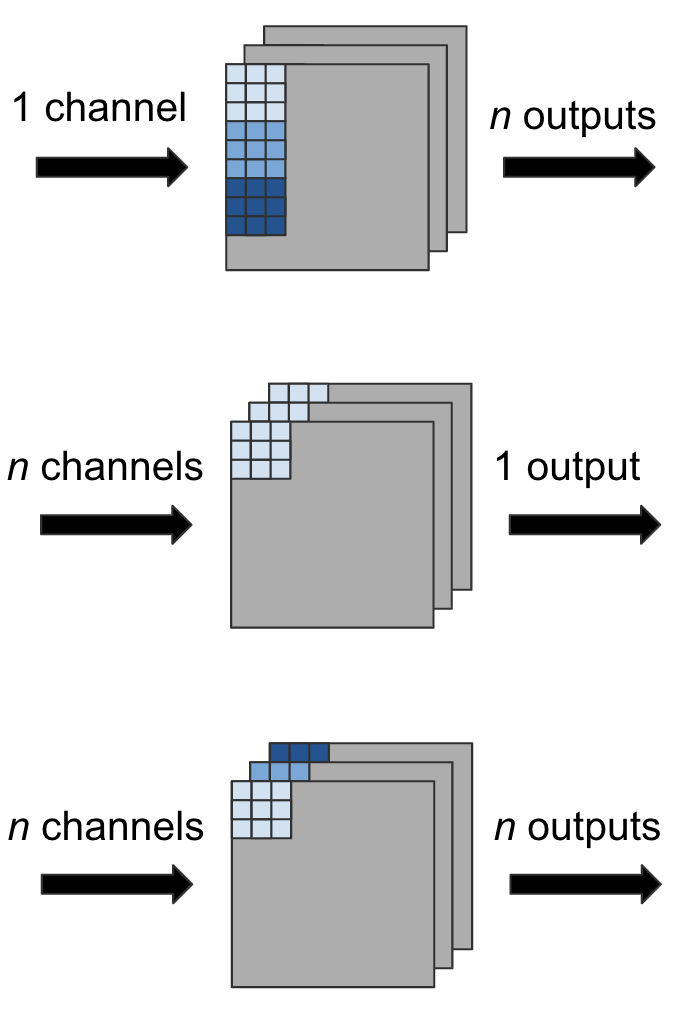
\includegraphics[scale=0.45]{ccu_parallelism}
	\caption[CCU Channel-Wise Parallelism]%
	{\narrower Channel-wise convolution oriented to either reuse inputs, outputs, or stay independent.}
	\label{ccuparallelism}
\end{wrapfigure}

Our CCU component computes a single channel's worth of convolution. \ref{ccuparallelism} shows how channel-wise parallelism can be oriented to either reuse inputs, outputs, or be entirely independent. In the case of reusing inputs, a mechanism must be in place to insure atomic updates are made to the output layer to prevent concurrent CCUs from overwriting values. In conjunction with one of these orientations, channel computation for a single input layer can be iterated to reuse existing input channels for different kernels altogether, or continue on the same kernel to complete the current output layer. Input and kernel sizes could drastically impact memory latencies for each orientation. Our work focuses primarily on the acceleration of a single CCU. Thus, we leave the exploration of CCU parallelism slated for future work.


\section{Environment and Experimental Results}
We implement our reconfigurable CCU against the Intel HLS Compiler. Benchmarks and correctness tests are obtained and verified using the ModelSim FPGA simulator. Each benchmark is ran using artificial data with input dimensionality and kernel sizes set to respective layer sizes from CNN architectures. Subsequent diagrams do not have a one-to-one correspondence with their actual hardware implementation due to the HLS translation. Floating point quantization is set to 16 bit precision throughout all implementations.

% ADD PART REGARDING MODEL SIM FPGA PARAMS LIKE MAKE, ETC

